
\section{Главный фактор загрязнения воздуха}
\begin{frame}{\insertsectionhead}
    \begin{minipage}{0.55\textwidth}
        \footnotesize
        Главным фактором загрязнения являются частицы с индексом
        PM2.5\cite{iqair}. 
        Это частицы вещества размером 2.5 мкм и менее.

        \medskip

        Данные частицы снижают ожидаемую продолжительность жизни 
        в среднем на 8.6 месяцев, вызывают аллергию, рак 
        и заболевания легких.
    \end{minipage}
    \begin{minipage}{0.43\textwidth}
        \hspace{1em}
        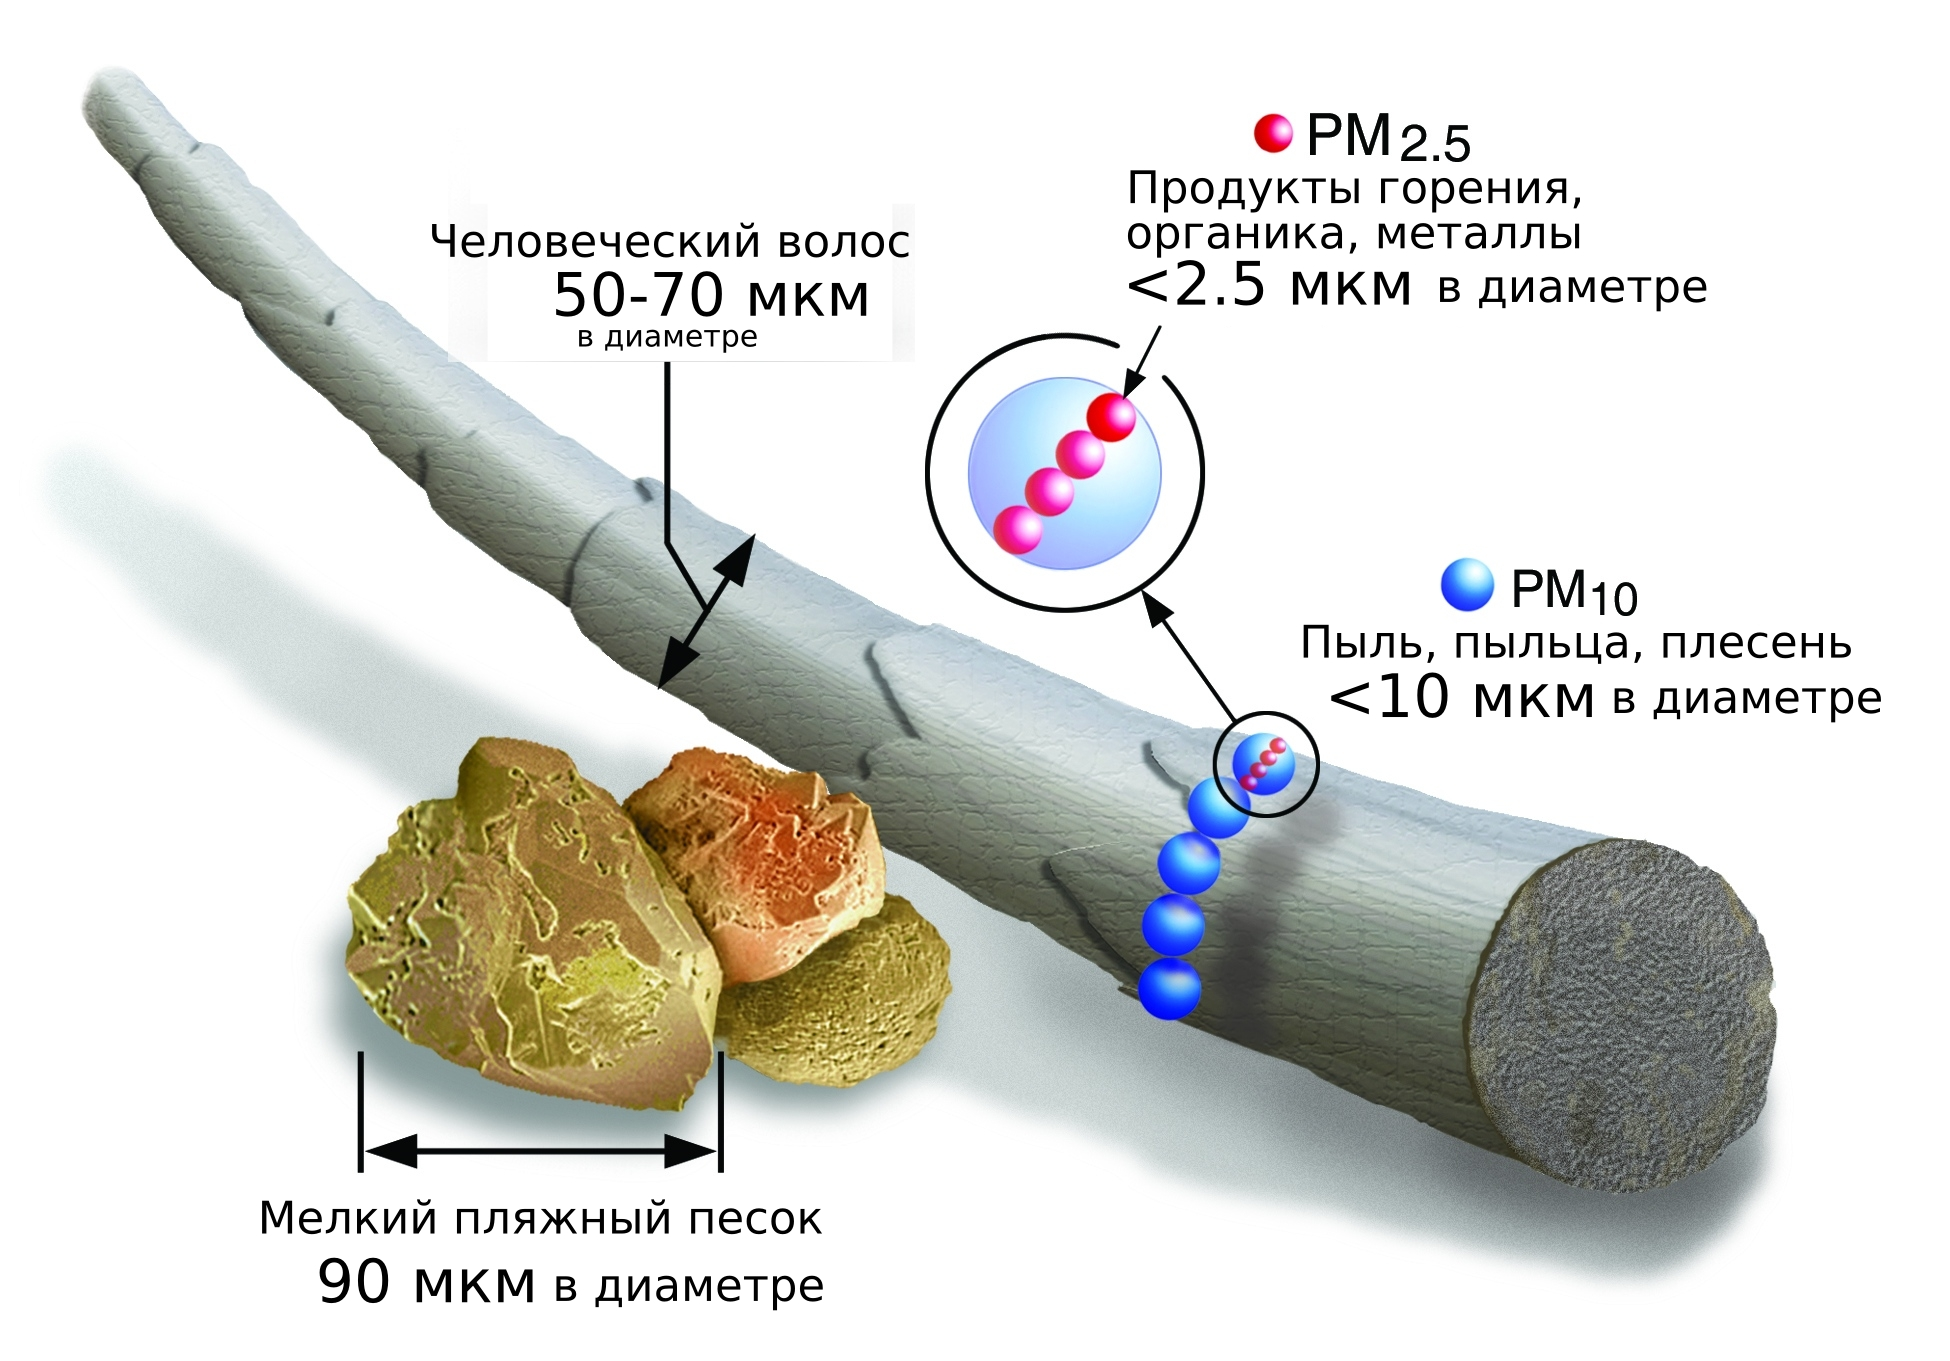
\includegraphics[width=\textwidth]{assets/pm25_scale_graphic.jpg}
    \end{minipage}
\end{frame}

